% Base de datos de la aplicación móvil
Se desea almacenar en el terminal móvil información referida a las solicitudes de recogida de muebles y enseres llevadas a cabo por el usuario de la aplicación, a fin de que este pueda consultarlas posteriormente las haya cursado. Dicha información sobre solicitudes incluirá información sobre las fechas (tanto de solicitud como de recogida), la ubicación donde acudirá el camión a recoger los enseres, y los enseres en si mismos que el usuario desea depositar. Dicha información además se empleará para poder gestionar el proceso de la solicitud de recogida de enseres permitiendo la clasificación de enseres en categorías y consultando todos los puntos de recogida de la localidad donde se preste servicio. \\
\begin{itemize}

\item \textbf{Enseres: }entre los enseres se incluyen tanto muebles como electrodomésticos de gran volumen que serán recogidos por el servicio de recogida y trasladados al punto limpio de la localidad. La organización desea información sobre los enseres para gestionar la recogida por parte del servicio de transporte. A cada enser en la aplicación móvil se le asociará un icono para mostrarlo al usuario. Los enseres serán identificados por un identificador único y contarán con un nombre.

\item \textbf{Punto de recogida: }representa los distintos puntos donde se depositan los muebles y enseres, Estos puntos coinciden con la ubicación de contenedores de otro tipo, y será la ubicación donde el camión llevará a cabo su parada para recoger dichos encere depositados previamente el usuario. De los puntos de recogida interesa conocer un identificador único, la localización en términos de latitud y longitud de cara a poder hacer uso de la tecnología gas del terminal móvil del usuario. Y como información aproximada la calle en la que se encuentre. Los puntos de recogida podrán ser de dos tipos: zonas cercanas al término municipal donde la recogida es diaria, y zonas alejadas del término municipal donde la recogida se realiza un día a la semana. Un punto de recogida tendrá un identificador numérico, y una localización que incluirá las coordenadas de longitud y latitud para su localización. Además del nombre de la calle en la que se encuentra. Aclarar que en una calle pueden existir varios puntos de recogida.

\item \textbf{Zona: }Se distingues a priori dos zonas distintas, las rurales y las urbanas. En las zonas urbanas la recogida se efectúa a día y para las zonas rurales hay un día para cada recogida. Podría ocurrir que en un futuro se incluyesen otras zonas. Las zonas vienen identificadas por una id y incluyen un nombre.

\item \textbf{Solicitudes de recogida: }toda solicitud de recogida incluye uno o varios enseres que serán recogidos en una o varias fechas. Además la solicitud va asociado un punto de recogida. La solicitud vendrá identificada por un valor numérico asociado a la solicitud llevada  a cabo por el usuario. Se incluirán dos fechas: por un lado la fecha de solicitud en la que el usuario contactó con el servicio de recogida de muebles y enseres y concertó la solicitud, y por otra parte la fecha de recogida asociadas a esa solicitud. 

\end{itemize}

\textbf{Restricciones semánticas} \
\
\begin{itemize}

\item Toda \textit{solicitud de recogida} tendrá de uno a cuatro {enseres} incluidos.

\item La \textit{fecha de solicitud} corresponderá al a fecha en la que se solicitó la recogida y la \textit{fecha de recogida} será posterior a esta y corresponderá a la fecha en la que se recogerán los muebles y enseres.

\item  La \textit{solicitud de recogida} se realizará en un único punto de recogida.

\item No existen dos \textit{puntos de recogida} con la misma \textit{localización}

\item No existen dos \textit{Zonas} con el mismo \textit{nombre}.

\end{itemize}

\textbf{Diagrama ER}

% Diagrama ER
\begin{figure}[H]
\centering
	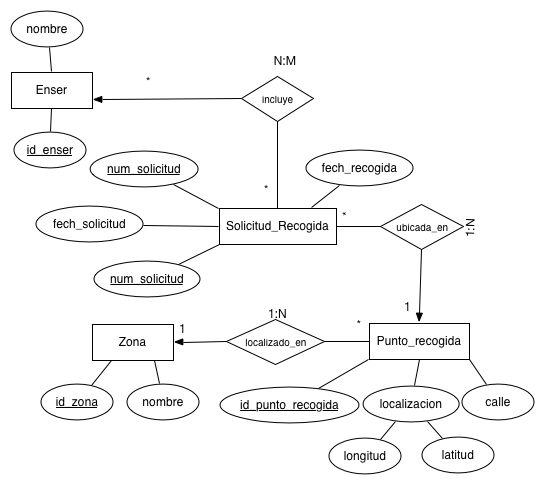
\includegraphics[scale=0.75]{bd-recicloid.png} 
  	 \caption{Diagrama ER de la base de datos de la aplicación móvil}
\end{figure}
